\documentclass[11pt]{article}
\usepackage{icmlko}
\begin{document}

\title{먼 손님이 아니라 눈이 어두운 손님이었다}
\author{월드모델 실험실}
\date{노트 435 · 2026년 8월 5일}
\maketitle

\begin{abstract}
노트 433이 ``다음 사이클의 첫 물음''으로 남긴 것 --- \emph{깊이 · lr · grp
셋 다 집 밖 짝 둘에서 크고 집안 LODO 열하나에서 없다. 까닭을 모른다.}
제일 그럴듯한 후보부터 쟀다: \textbf{거리}.

\begin{center}
\begin{tabular}{lr}
\hline
거리 $\leftrightarrow$ grp 이득 ($n{=}13$) & $\rho = \mathbf{-0.203}$ \\
집안 열하나의 평균 거리 & $0.7420$ \\
\textbf{집 밖 둘의 평균 거리} & $\mathbf{0.4618}$ \\
\hline
\end{tabular}
\end{center}

\textbf{반증됐다. 그것도 거꾸로.} KR 만화($0.400$)와 비게임 앱($0.524$)은
열세 중 \textbf{가까운 축}이고 애니($1.341$) · 모바일($1.039$)이 제일 멀다.
\textbf{``집 안팎''이라는 이름부터 틀렸다} --- 그 둘은 멀어서 유난한 것이
아니다.

그러면 무엇이 다른가. 열어 보니 하나 있었다. \textbf{KR 만화와 비게임 앱은
공유 축 다섯만 채워져 있다} --- 나머지 스물아홉 열은 중립 $0.5$ · 표시자 $0$
이다. LODO 도메인은 제 축을 다 갖는다(게임 유보에서 관측 축 15 · 아이돌 15 ·
모바일 17). \textbf{모델이 볼 것이 적을수록 도메인 표지가 크게 산다}면 그
둘이 유난한 것이 설명된다.
\end{abstract}

\section{축을 줄여 봤다}

LODO 도메인의 \textbf{예측 때} 축을 공유 다섯으로 가리고 grp 이득을 다시 쟀다.
학습은 그대로다.

\begin{center}
\begin{tabular}{lrr}
\hline
 & 원래 & 축 줄임 \\
\hline
\textbf{LODO 열한 짝 평균} & $-0.0004$ & $\mathbf{+0.0152}$ \\
아이돌 & $-0.0921$ & $\mathbf{+0.1226}$ \\
애니 & $+0.0462$ & $\mathbf{+0.1222}$ \\
웹툰 & $-0.0069$ & $-0.0801$ \\
펀딩 & $-0.0446$ & $-0.0778$ \\
\hline
집 밖 둘 & \multicolumn{2}{c}{KR $+0.2950$ · 앱 $+0.1053$} \\
\hline
\end{tabular}
\end{center}

\textbf{사전 등록 통과} --- 평균이 커지고 양수가 됐다. 아이돌은 $-0.092$ 에서
$+0.123$ 으로 \textbf{부호가 뒤집힌다}(관측 축 15 중 12를 가렸다). 애니도
두 배 넘게 는다.

\textbf{그러나 절반만이다.} 부호 셈은 $5/11$ 그대로이고, 평균 $+0.0152$ 는
집 밖 둘($+0.105$ · $+0.295$)에 한참 못 미친다. 웹툰과 펀딩은 오히려 더
내려간다.

\section{가림이 진짜 가렸는지 확인했다}

숫자가 이상한 데가 있었다 --- 게임의 grp 팔이 가리기 전후로 $0.5125$ 로
소수점 넷째 자리까지 같았다. 열어 봤다.

\begin{center}
\begin{tabular}{lrr}
\hline
 & 유보 관측 축 & 가린 축 \\
\hline
게임 & $15$ & $\mathbf{10}$ \\
아이돌 & $15$ & $\mathbf{12}$ \\
시장팝업 & $3$ & $0$ \\
팝업 & $5$ & $0$ \\
\hline
\end{tabular}
\end{center}

가림은 제대로 돈다. 시장팝업과 팝업은 \textbf{원래 축이 다섯 이하라 진짜
아무 일도 안 일어나고}, 그 둘의 이득이 소수점까지 그대로인 것($-0.0017$ ·
$+0.0213$)이 그 증거다. 게임은 열 개를 가렸는데 값이 같았다 --- 우연이다.

\section{그래서 어디까지 왔나}

\begin{itemize}
\item \textbf{거리는 아니다.} 그리고 집 밖이 더 가깝다 --- 이름을 고쳐야 한다.
\item \textbf{축의 개수가 일부다.} 눈을 가리면 표지가 커진다. 평균이
$-0.0004 \to +0.0152$, 아이돌은 부호가 뒤집힌다.
\item \textbf{전부는 아니다.} $+0.20$ 까지 못 가고 웹툰·펀딩은 반대로 간다.
\end{itemize}

남은 차이는 라벨 계기 · 수집 절차 · 언어처럼 \textbf{지금 자료로 못 가르는
것}들이다. 노트 424가 ``두 자리''에서 멈춘 것과 같은 자리다.

\begin{tabular}{lp{7.0cm}}
\hline
축 개수를 눈금으로 & 이제 ``관측 축 수''가 전이 이득의 예보에 쓰일 수 있다.
노트 411이 못 간 길이 반쯤 열렸다 \\
웹툰 · 펀딩 & 축을 줄이면 더 나빠지는 둘. 노트 414의 웹툰이 또 나온다 \\
집 밖 셋째 & 축 다섯짜리가 아닌 집 밖 도메인이 있어야 두 요인을 가른다 \\
\hline
\end{tabular}

\begin{figure}[h]
\centering
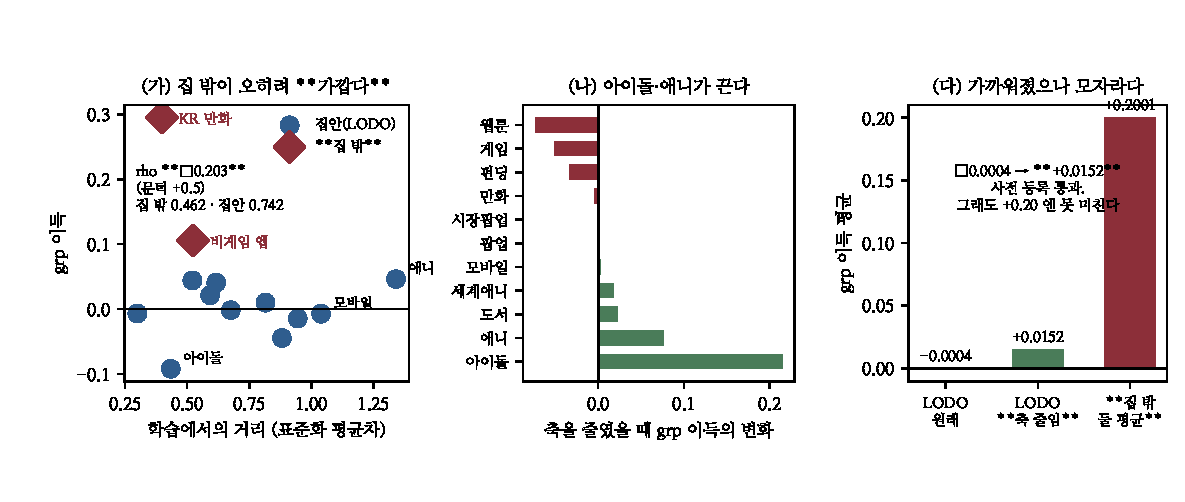
\includegraphics[width=\textwidth]{figs/fig435.pdf}
\caption{(가) 거리는 반대로 나온다 --- 집 밖이 가깝다. (나) 축을 줄였을 때
이득의 변화. (다) 평균이 집 밖 쪽으로 가지만 못 미친다.}
\end{figure}

\end{document}
